\frame{%
\frametitle{Summary}
\begin{itemize}
\item Decision theory and expected utility
\begin{itemize}
\item Very brief introduction
\item Why expected utility?
\end{itemize}
\pause
\item Decision making in health economics
\begin{itemize}
\item Statistical framework
\item Running example
\item Choosing a utility function
\end{itemize}
\pause
\item Cost-effectiveness analysis
\begin{itemize}
\item Running example
\item Expected Incremental Benefit
\item Cost-effectiveness plane (revisited)
\end{itemize}
\end{itemize}

\vfill
{\footnotesize  \emph{Bayesian Methods in Health Economics} (BMHE), chapter 3.1 --- 3.3}

}

\frame{
\frametitle{Decision theory}
\begin{itemize}
\item Health economic evaluations are a typical example of decision problem
\begin{itemize}
\item Assess whether a new intervention (treatment) $t=1$ should be selected to replace a current standard of treatment $t=0$
\item Basically need to identify whether the potential gains in health provided by switching the population to $t=1$ more than offset the potential increase in costs
\end{itemize}
\item Of course, we need to decide in the \alert{face of uncertainty}
\begin{itemize}
\item Both costs \& consequences of a given intervention are \textbf{unknown} as they will fully occur (or not) in the future
\end{itemize}
\end{itemize}

\vspace{5pt}
\textbf{Objectives}
\begin{itemize}
\item Set the framework for rational decision-making
\item Define decision criteria
\end{itemize}
}

\frame{
\frametitle{Decision theory}
\textbf{Basic elements}
\begin{itemize}
\item A set of possible \alert{decisions}
\begin{itemize}
\item $t \in \mathcal{T}$ --- alternatives available to the decision-maker (DM)
\item We may consider $\mathcal{T}=(0,1)$ (standard vs innovative treatment)
\end{itemize}
\vspace{10pt}\pause
\item A set of \alert{consequences} (outcomes) associated with each intervention
\begin{itemize}
\item $o \in \mathcal{O}$. \textbf{NB}: These will depend on a set of \textbf{\blue random quantities} $\bm\omega \in \Omega$
\item $o = (\bm\omega,t)$ = the result of applying $t$ if future unfolds according to $\bm\omega$
\item In other words, $\mathcal{O} = \Omega\times\mathcal{T}$
\end{itemize}
\vspace{10pt}\pause
\item A scheme of \alert{preferences}
\begin{itemize}
\item $t_1\preceq t_2 \Rightarrow$ the random consequences of $t_1$ are not preferred to those of~$t_2$
\item $t_1\sim t_2 \Rightarrow$ the two actions are indifferent
\end{itemize}
\end{itemize}
}

\frame{
\frametitle{Decision theory}
\textbf{Prescriptive axioms}
\begin{itemize}
\item Comparability of consequences
\begin{itemize}
\item The DM is capable of ranking the interventions, based on their consequences
\end{itemize}
\item Transitivity of preferences
\begin{itemize}
\item Cannot have circular preferences ($t_1\preceq t_2$, $t_2\preceq t_3$, $t_3\preceq t_1$)
\end{itemize}
\item Consistency of preferences
\begin{itemize}
\item ``Sure-thing principle''
\end{itemize}
\item Quantifiability of preferences
\begin{itemize}
\item Assumes the existence of standard ``reference'' for comparison
\end{itemize}
\end{itemize}
\vspace{10pt}
\textbf{NB}: If the DM acts in a way that these hold, then s/he is rational $\Rightarrow$ always takes the ``optimal'' decision, based on the current knowledge
}

\frame{
\frametitle{(Bayesian) Decision theory}
Bayesian decision theory prescribes that
\begin{itemize}
\item Uncertainty is described by means of a (\textbf{possibly} subjective) \alert{probability distribution} $p(\bm\omega)$
\begin{itemize}
\item $p:\Omega \rightarrow [0;1]$ --- associates a number in $[0;1]$ to each random quantity
\end{itemize}
\item Outcomes are valued by means of a \alert{measure of utility} $u(o)=u(\bm\omega,t)$
\begin{itemize}
\item $u:\mathcal{O}\rightarrow \mathbb{R}$ --- associates a real number to each consequence (eg via standard gamble)
\end{itemize}
\vspace{7pt}
\item Typically, $\bm\omega=(y,\bm\theta)$
\begin{itemize}
\item $y=(e,c)$ = observable future results (eg occurrence of disease; costs)
\item $\bm\theta$ = relevant parameters, indexing the distribution of $y$ (eg population probability of cancer; average cost, etc)
\item $p(\bm\omega) = p(y,\bm\theta) = \color{red}p(y\mid \bm\theta)\color{blue}p(\bm\theta)$
\item[] $\phantom{p(\bm\omega) = p(y,\bm\theta)}$ = \color{red}observable data model \color{black}$\times$ \color{blue}model for prior knowledge\color{black}
\end{itemize}
\vspace{7pt}
\item Outcomes $o$ = observable variables $y$
\begin{itemize}
\item Thus $o=(y,t)$ and the associated utility measure is $u(y,t)$
\end{itemize}
\end{itemize}
}

%%%\frame{
%%%\frametitle{Assigning utilities (standard gamble)}
%%%
%%%\usetikzlibrary{trees,shapes}
%%%\tikzstyle{decision} = [rectangle, minimum height=8pt, minimum width=8pt, draw=blue!10, fill=solid, ultra thick, inner sep=0pt]
%%%\tikzstyle{chance} = [circle, minimum width=8pt, draw=blue!10, fill=solid, ultra thick, inner sep=0pt]
%%%\tikzstyle{line} = [draw=none]
%%%\tikzstyle{end} = [diamond, minimum width=6pt, minimum height=6pt, fill=none, inner sep=0pt, draw=red, thin]
%%%\tikzset{
%%%grow=right,
%%%join=miter,
%%%level 1/.style={sibling distance=2cm, level distance=3.8cm},
%%%level 2/.style={sibling distance=2cm, level distance=3.0cm},
%%%level 3/.style={sibling distance=2cm, level distance=5.5cm},
%%%edge from parent/.style={thick, draw=black},
%%%edge from parent fork right,
%%%every node/.style={text centered, inner sep=1cm}
%%%align=center,
%%%anchor=north
%%%}
%%%
%%%\begin{center}
%%%\begin{tikzpicture}[]
%%%\small
%%%\node[decision]{}
%%%    child{node[line]{$\red y_s$}
%%%      edge from parent 
%%%        node[above,near end]{Option 2}
%%%        node[below,near end]{\myblue 1}
%%%    }
%%%    child{node[chance]{}
%%%      child{node[line]{\red $y_w$}
%%%       edge from parent
%%%         node[below,near end]{$\myblue  1-\pi_s$}
%%%      }
%%%      child{node[line]{$\red y_b$}
%%%       edge from parent
%%%         node[below,near end]{$\myblue \pi_s$}
%%%      }
%%%      edge from parent
%%%            node[above,near end]{Option 1}
%%%    };
%%%    \node[fill=none] at (5.0,-1.1) {\fontsize{8}{8}\selectfont $\black \leadsto \orange u(y_s,t)=\pi_s$};
%%%    \node[fill=none] at (8.0,1.7)  {\fontsize{8}{8}\selectfont $\black \leadsto \orange u(y_b,t)=1$};
%%%    \node[fill=none] at (8.0,-0.3) {\fontsize{8}{8}\selectfont $\black \leadsto \orange u(y_w,t)=0$};
%%%\end{tikzpicture}
%%%\end{center}
%%%
%%%\begin{itemize}
%%%\item Define the ``best'' and ``worst'' \red{outcomes} \black (say, $\red y_b$ and $\red y_w$) 
%%%\item Associate utility \orange 1 \black and \orange 0 \black respectively with $\red y_b$ and $\red y_w$
%%%\item Evaluate comparatively any other outcome $\red y_s$
%%%\begin{itemize}
%%%\item Exchange $\red y_s$ with \myblue certainty\black\ (\ie probability \myblue 1\black ) with an uncertain scenario in which $\red y_b$ is obtained with probability $\myblue  \pi_b$ --- but $\red y_w$ is obtained with probability $\myblue (1-\pi_s)$!
%%%\item Associate utility $\orange \pi_s$ with $\red y_s$
%%%\end{itemize}
%%%\end{itemize}
%%%}

\frame{
\frametitle{(Bayesian) Decision theory --- decision criterion}
\textbf{Objective}
\begin{itemize}
\item Determine a general criterion to base decision on
\item Intuitively, select the option associated with the highest chance of producing the preferred outcome (consequence)
\end{itemize}
\vspace{10pt}
\textbf{Result}
\begin{itemize}
\item As it turns out, \alert{the chance of obtaining the preferred outcome %$y^{\rm{max}}$ 
is maximised if the expectation of the utility measure is maximised}
\begin{itemize}
\item \textbf{NB}: dealing with expectations is in general much simpler than dealing with probability assessment!
\item Moreover, because of this equivalence, expectation is the only quantity we should worry about --- \textbf{based on current knowledge}, no need to assess variability (but more on this later!)
\end{itemize}
\end{itemize}
}

%%%\frame{
%%%\frametitle{Example --- expected utility}
%%%\begin{itemize}
%%%\item Two alternative interventions: $t=0,1$
%%%\item $S=4$ health states, valued by the SF-6D (see Lecture 1)
%%%\begin{itemize}
%%%\item $y_1 = \texttt{111111}$ (perfect health --- preferred outcome, $u(y_1,t):=1$)
%%%\item $y_2 = \texttt{433433}$
%%%\item $y_3 = \texttt{645655}$
%%%\item $y_4 = $ death (least favourite outcome, $u(y_4,t):=0$)
%%%\end{itemize}
%%%\item $\bm\theta^t=(\theta^t_1,\ldots,\theta^t_S)$ = probability of obtaining state $s$ under treatment $t$
%%%\begin{itemize}
%%%\item For simplicity, unrealistically assume them known with no uncertainty
%%%\end{itemize}
%%%\vspace{10pt}\pause
%%%\item The preferred outcome can be obtained in either of these
%%%\begin{enumerate}
%%%\item \alert{directly}: if $y_1$ obtains, with probability $\theta^t_1$
%%%\item \alert{virtually}: by definition of utilities, any other state $y_s$ is equivalent to a scenario where perfect health is obtained with probability $\pi_s = u(y_s,t)$
%%%\end{enumerate}
%%%\end{itemize}
%%%}
%%%
%%%\frame{
%%%\frametitle{Example --- expected utility}
%%%Consequently
%%%\myblue
%%%\begin{eqnarray*}
%%%\Pr(y_1 \mid \bm\theta^t) & = & \theta^t_1 + \sum_{s=2}^S \pi_s \Pr(y_s \mid \bm\theta^t_s) \\
%%%& = & \sum_{s=1}^S \pi_s \times \theta^t_s =  \sum_{s=1}^S u(y_s,t)\times \theta^t_s \\
%%%& = & \mbox{E}[u(Y,t)] = \mathcal{U}^t = \mbox{\textbf{expected utility}}
%%%\end{eqnarray*}
%%%\black \vspace{-10pt} \pause
%%%
%%%Of course, in general, we do not know $\bm\theta^t$ without uncertainty and $y$ may be a continuous random variable and thus
%%%\[ \mathcal{U}^t = \int\int u(y,t)p(y\mid\bm\theta^t)p(\bm\theta^t)\mbox{d}y\mbox{d}\bm\theta^t \]
%%%
%%%\vspace{5pt}
%%%\textbf{NB}: $u:\Omega\times\mathcal{T}\rightarrow \mathbb{R}$ while $\mathcal{U}:\mathcal{T}\rightarrow \mathbb{R}$ (\blue marginalisation of uncertainty\black)
%%%}

\frame{
\frametitle{Statistical framework}
\begin{itemize}
\item \alert{Health economic response}: $(e,c)$
\begin{itemize}
\item $\myblue e$ = a measure of clinical benefit (eg QALYs)
\item $\myblue c$ = the total cost associated with each intervention
\end{itemize}
\vspace{10pt}\pause
\item \alert{Treatment-specific population parameter} $\bm\theta^t$
\begin{itemize}
\item Probability of some clinical outcome
\item Duration in treatment
\item Reduction in the occurrence of some event
\end{itemize}
\vspace{10pt}\pause
\item (\textbf{At least}) \alert{Two sources of uncertainty}
\begin{itemize}
\item \color{red}Sampling variability \color{black}is modelled using an intervention-specific distribution $\color{myblue}p(e,c \mid \bm\theta^t)$
\item \color{red} Parametric uncertainty \color{black}is modelled using a (possibly subjective) prior distribution $\color{myblue} p(\bm\theta^t\mid\mathcal{D})$, based on some background data $\mathcal{D}$
\item \textbf{NB}: Sometimes, we can (should!) consider also \color{red} structural uncertainty\color{black}, i.e.\ about the modelling assumptions used (\textbf{more on this later!})
\end{itemize}
\end{itemize}
}

\frame{
\frametitle{Choosing a utility function}
\begin{itemize}
\item Typically, we do health economic evaluation based on the \alert{monetary net benefit}
\[ \myblue u(e,c;t):=ke - c \] \vspace{-15pt}
\begin{itemize}
\item $k$ is the ``willingness to pay'', i.e.\ the \textit{\red cost per extra unit of effectiveness gained}
\end{itemize}
\vspace{10pt}\pause
\item The main advantages of using the MNB are that
\begin{itemize}
\item It has a fixed form, once $e,c$ are observed
\item It is a \alert{linear} function in $e,c$, which simplifies computations
\end{itemize}
\vspace{10pt}\pause
\item However, MNB presupposes that the DM is \textit{risk neutral}
\begin{itemize}
\item Non necessarily true --- \textbf{more on this later!}
\end{itemize}
\end{itemize}
}

\frame{
\frametitle{Bayesian decision-making}
\begin{enumerate}
\item For each intervention $t$, compute the \textit{\red expected utility} \vspace{-5pt} \[\myblue \mathcal{U}^t = \mbox{E}[u(e,c;t)] \] \vspace{-15pt}
\begin{itemize}
\item \textbf{NB}: This is done with respect to \textbf{both} individual and population uncertainty
\item Hence $\mathcal{U}^t$ is a pure number!
\end{itemize} \pause\vspace{10pt}
\item Treat the \textit{entire} homogeneous (sub)population with the most cost-effective treatment, (maximum expected utility)
\begin{itemize}
\item \textbf{NB}: Equivalently, if $\mathcal{T}=(0,1)$, then $t=1$ is the most cost-effective intervention if the \textbf{\blue Expected Incremental Benefit} is positive
\end{itemize}\vspace{5pt}
\[ \myblue \mbox{EIB}=\mathcal{U}^1-\mathcal{U}^0 > 0 \Rightarrow \mbox{$t=1$ is more cost-effective }\]
\pause\vspace{-10pt}
\item Perform \textbf{\red sensitivity analysis} (to parameter and/or structural uncertainty) to investigate the impact of underlying uncertainty on the decision process
\end{enumerate}
}

\frame{
\frametitle{Bayesians do it better!}
\begin{itemize}
\item Ideal to build decision models 
\begin{itemize}
\item Often based on evidence synthesis (\textbf{more on this in Lecture \ref{Hierarchical1}!})
\end{itemize}
\item Include knowledge and push uncertainty through
\begin{itemize}
\item Probabilistic sensitivity analysis (\textbf{more on this in Lecture \ref{PSALecture}!})
\end{itemize}
\item Very good to deal with individual level data too
\begin{itemize}
\item Easy to model the joint outcome $(e,c)$
\item Can account for excess of zero costs or bimodality in the utility measures (\eg using mixture models)
\end{itemize}
\end{itemize}

\onslide<2|handout:0>{

\includegraphics[scale=.18]{5.statistical-cost-effectiveness-analysis/figs/Madonna}}
}

\frame{
\frametitle{EIB vs ICER}
\begin{itemize}
\item Recall that
\[ \myblue \mbox{ICER} = \frac{\mbox{E}[\Delta_c]}{\mbox{E}[\Delta_e]} = \mbox{\black Additional cost to gain 1 unit of benefit} \]
\begin{itemize}
\item $\myblue \Delta_e=\red\underbrace{\myblue\mbox{E}[e \mid \theta^1]}_{\mu_1^e} \myblue - \red\underbrace{\myblue\mbox{E}[e \mid \theta^0]}_{\mu_0^e}$ = increment in mean benefits
\item $\myblue \Delta_c=\red\underbrace{\myblue\mbox{E}[c \mid \theta^1]}_{\mu_1^c} \myblue - \red\underbrace{\myblue\mbox{E}[c \mid \theta^0]}_{\mu_0^c}$ \hspace{1pt}= increment in mean costs
\item \textbf{NB}: Both depend on $\bm\theta^t$, which is a random variable!
\end{itemize}
\vspace{20pt}\gray
\item[\gray $\bullet$] When the MNB is used as utility function and $\mathcal{T}=(0,1)$
\[ \mbox{EIB} = \mathcal{U}^1-\mathcal{U}^0=\mbox{E}[k\Delta_e - \Delta_c] = k\mbox{E}[\Delta_e] - \mbox{E}[\Delta_c] \]
and thus
\[ \mbox{EIB}>0 \Rightarrow k>(<)\frac{\mbox{E}[\Delta_c]}{\mbox{E}[\Delta_e]} = \mbox{ICER} \quad \mbox{if $\mbox{E}[\Delta_e]>(<)0$}\]
\end{itemize}
}

\frame{
\frametitle{Cost effectiveness plane vs.\ ICER}
\begin{figure}
\begin{tikzpicture}
\node{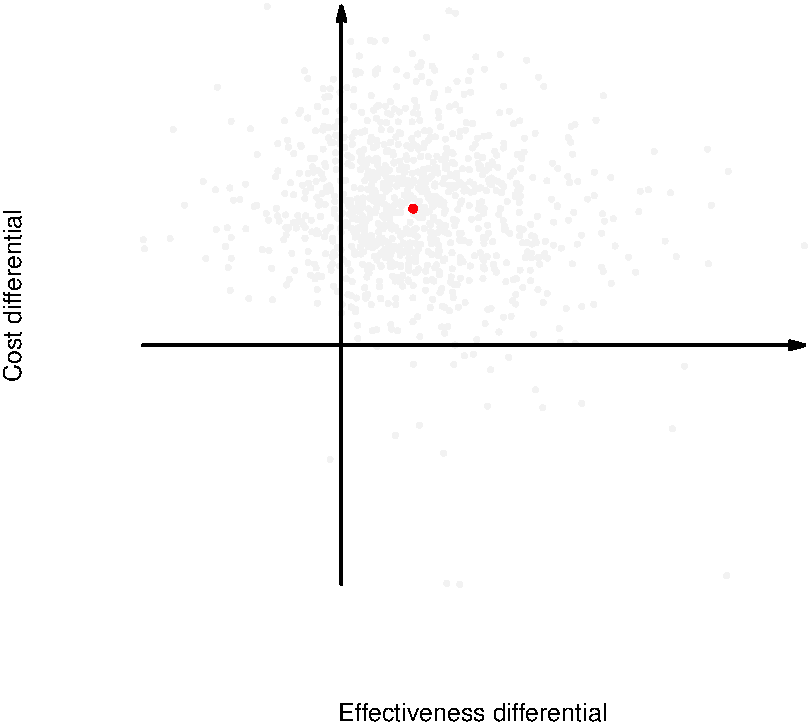
\includegraphics[scale=.55]{1.introduction-to-health-economic-evaluations/figs/CEPlane_ICER}};
\draw(3.5,-.1) node[align=center,rectangle,rounded corners,draw=none,text width=4.1cm](8){\fontsize{8}{8}\selectfont $\Delta_e$};
\draw(-.9,3.2) node[align=center,rectangle,rounded corners,draw=none,text width=4.1cm](8){\fontsize{8}{8}\selectfont $\Delta_c$};
\draw(2.5,1.6) node[align=center,rectangle,rounded corners,draw=none,text width=6.0cm](8){\fontsize{8}{8}\selectfont $\mbox{ICER}=\frac{\mbox{E$[\Delta_c]$}}{\mbox{E$[\Delta_e]$}}=\mbox{Cost per QALY}$};
\end{tikzpicture}
\end{figure}
}


\frame{
\frametitle{EIB vs ICER}
\begin{itemize}
\item[\gray $\bullet$]\gray Recall that
\[ \mbox{ICER} = \frac{\mbox{E}[\Delta_c]}{\mbox{E}[\Delta_e]} = \mbox{Additional cost to gain 1 unit of benefit} \]
\begin{itemize}
\item[\gray $\bullet$] $\gray\Delta_e=\underbrace{\mbox{E}[e \mid \theta^1]}_{\mu_1^e} - \underbrace{\mbox{E}[e \mid \theta^0]}_{\mu_0^e}$ \gray = increment in mean benefits
\item[\gray $\bullet$] $\gray\Delta_c=\underbrace{\mbox{E}[c \mid \theta^1]}_{\mu_1^c} - \underbrace{\mbox{E}[c \mid \theta^0]}_{\mu_0^c}$ \gray\hspace{1pt}= increment in mean costs
\item[\gray $\bullet$] \textbf{NB}: Both depend on $\bm\theta^t$, which is a random variable!
\end{itemize}
\vspace{20pt} 
\item \black When the MNB is used as utility function and $\mathcal{T}=(0,1)$
\[ \myblue \mbox{EIB} = \mathcal{U}^1-\mathcal{U}^0=\mbox{E}[k\Delta_e - \Delta_c] = k\mbox{E}[\Delta_e] - \mbox{E}[\Delta_c] \]
and thus
\[ \myblue \mbox{EIB}>0 \Rightarrow k>(<)\frac{\mbox{E}[\Delta_c]}{\mbox{E}[\Delta_e]} = \mbox{ICER} \quad \mbox{if $\mbox{E}[\Delta_e]>(<)0$} \]
\end{itemize}
}

\frame{
\frametitle{Cost-effectiveness plane vs EIB vs ICER}
\begin{center}
\only<1|handout:1>{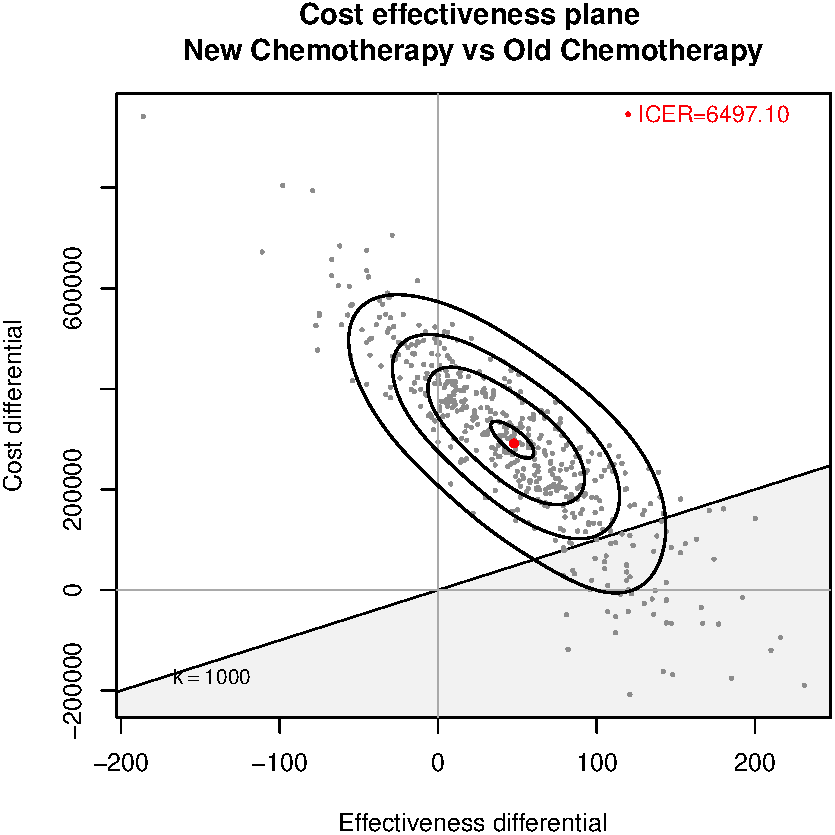
\includegraphics[width=7.6cm]{5.statistical-cost-effectiveness-analysis/figs/contour2_2}}
\only<2|handout:2>{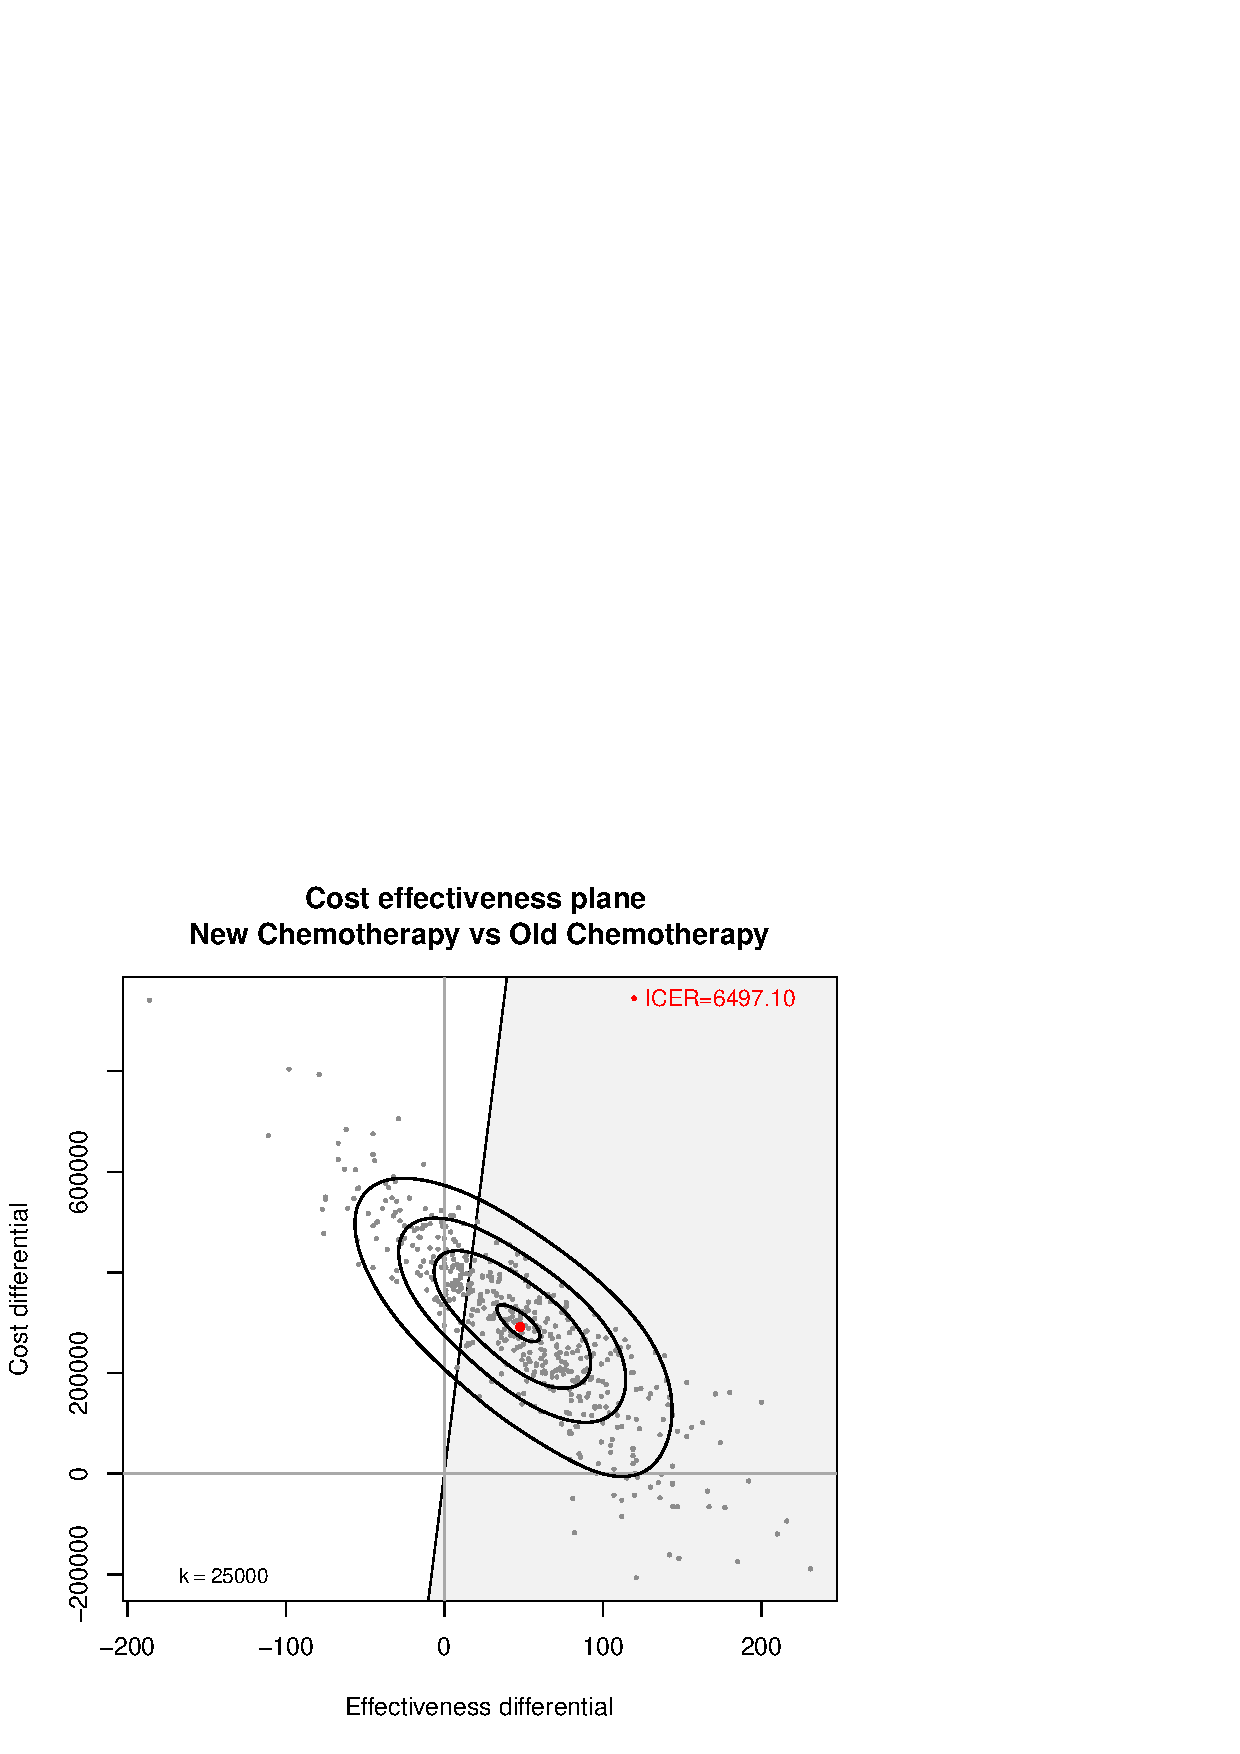
\includegraphics[width=7.6cm]{5.statistical-cost-effectiveness-analysis/figs/contour2}}
\end{center}
}

\frame{
\frametitle{So: problem solved?}
\textbf{\red ... Well, not really!}\pause
\begin{itemize}
\item The quality of the current evidence is often limited
\begin{itemize}
\item During the pre-market authorisation phase, the regulator should decide whether to grant reimbursement to a new product --- and in some countries also set the price --- on the basis of uncertain evidence, regarding both clinical and economic outcomes
\end{itemize}
\vspace{5pt}
\pause
\item This leads to the necessity of performing \textit{\myblue{(probabilistic) sensitivity analysis}~\textbf{(PSA)}} --- \textbf{more on this in lecture \ref{PSALecture}} 
\begin{itemize}
\item Formal quantification of the impact of uncertainty in the parameters on the results of the economic model
\item Standard requirement in many health systems (e.g.\ for NICE in the UK), but still not universally applied
\item Often limited to \textit{\red parametric} uncertainty, but should be extended to \textit{\blue structural} uncertainty too (\textbf{more on this in lecture \ref{StructPSA}})
\end{itemize}
\end{itemize}
}
%%%%%%
%%%%%%\frame{
%%%%%%\frametitle{The rationale for PSA}
%%%%%%\vspace{-5pt}
%%%%%%\begin{itemize}
%%%%%%\item Identify the best course of action \textbf{given the current level of information}
%%%%%%\item Evaluate how the decision is influenced by the potential reduction in uncertainty about the parameters (eg new data)
%%%%%%\end{itemize}
%%%%%%\begin{center}
%%%%%%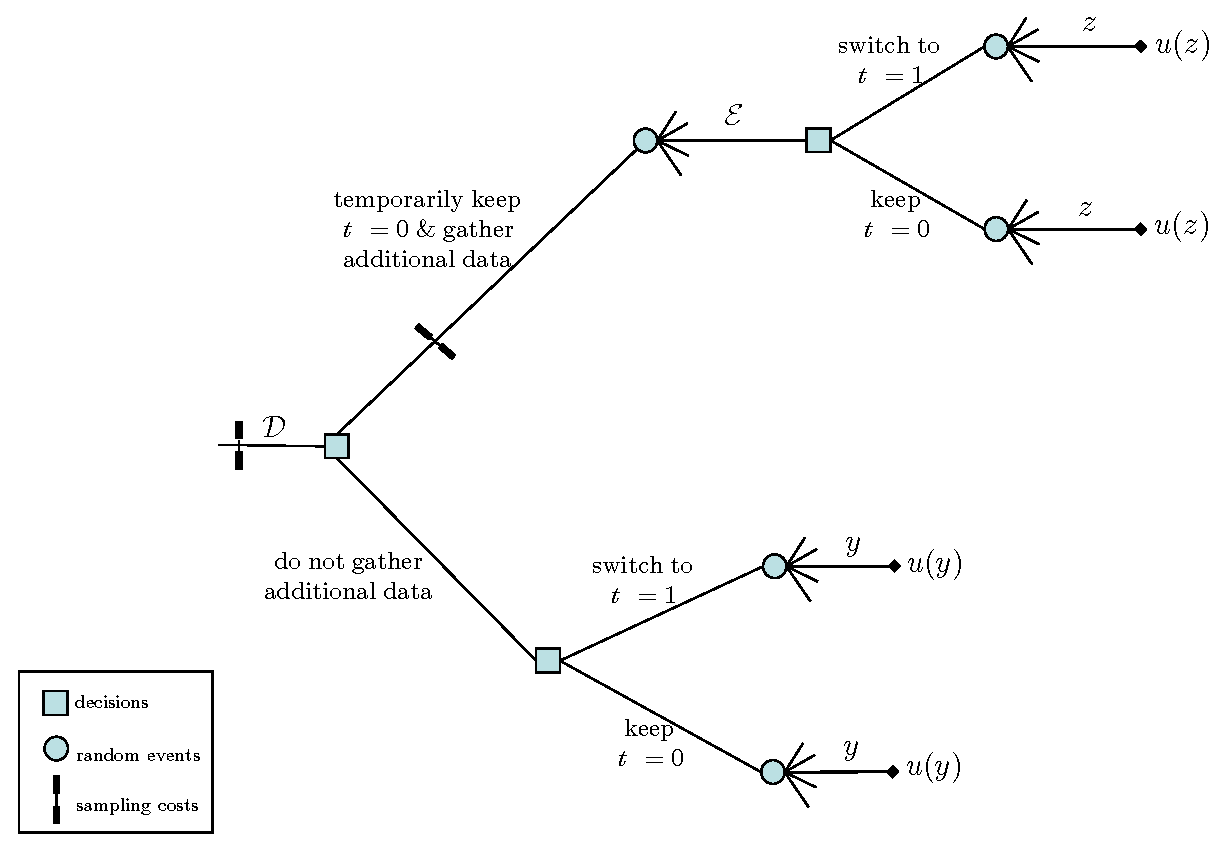
\includegraphics[scale=.4]{5.statistical-cost-effectiveness-analysis/figs/PSA_Tree}
%%%%%%\end{center}
%%%%%%}

\frame{%
\frametitle{\bcea: a package for Bayesian health economics}%
\textbf{\myblue What is \bcea \textbf{not}?}
\begin{itemize}
\item \bcea is \textbf{not} a package to automatically run a Bayesian analysis
\begin{itemize}
\item It cannot build the health economic model for you
\item It does not prepare the data to be used in the model
\item It does not automatically run the MCMC simulations
\item It does not choose the prior distributions for you
\end{itemize}
\end{itemize}

\vspace{5pt}\pause
\textbf{\myblue So what \textrm{\textit{is}} it, then?}%
\begin{itemize}
\item \bcea provides a set of specific functions to systematically post-process the output of a Bayesian health economic model
\item Uses \R (\texttt{\myblue http://cran.r-project.org/})
\begin{itemize}
\item Very good at interacting with standard MCMC software
\item[] $\bullet$ \texttt{BUGS} (\texttt{\myblue www.mrc-bsu.cam.ac.uk/bugs/winbugs/contents.shtml})
\item[] $\bullet$ \texttt{JAGS} (\texttt{\myblue www.mcmc-jags.sourceforge.net/})
\item \textbf{\red Free} and there is a very large community of contributors
\item Specifically designed for statistical analysis and has very good graphical capabilities
\end{itemize}
\end{itemize}
}

\frame{
\frametitle{The \texttt{R} package \texttt{BCEA}}
\begin{figure}
\centering
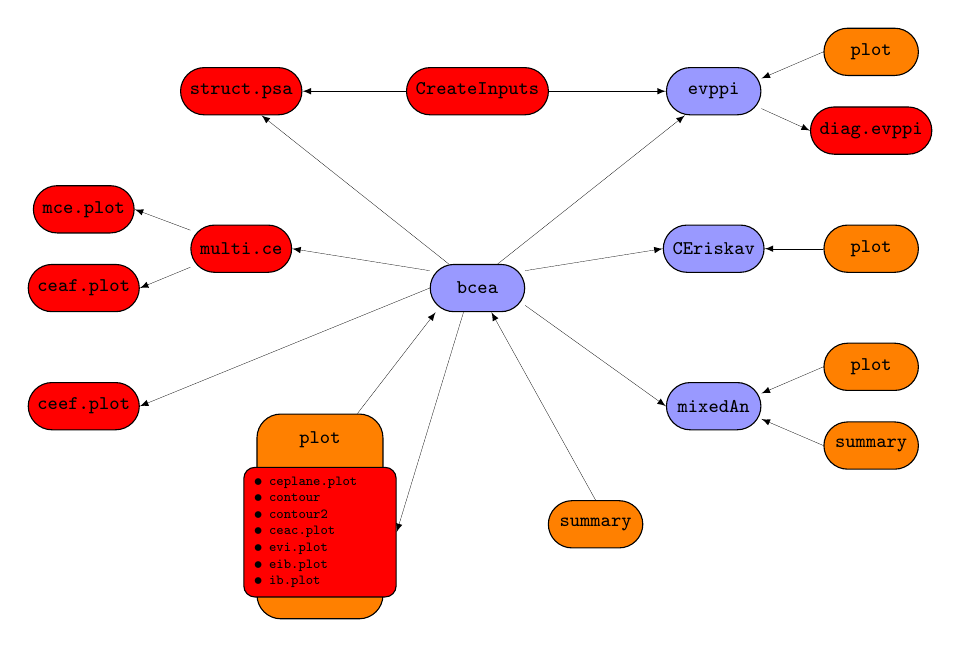
\begin{tikzpicture}

\draw(0,0) node[align=center,rectangle,rounded corners=2ex,draw,fill=blue!40,font=\sffamily\fontsize{7}{8}\selectfont,minimum width=1.2cm,minimum height=.6cm](1){\texttt{bcea}};

\draw(-2,-2.9) node[align=center,rectangle,rounded corners=2ex,draw,fill=orange,font=\sffamily\fontsize{7}{8}\selectfont,minimum width=1.6cm,minimum height=2.6cm,text depth=2.0cm](2){\texttt{plot}};

\draw(-2.0,-3.1) node[align=left,rectangle,rounded corners,draw,fill=red,font=\sffamily\fontsize{6}{7}\selectfont,text width=1.7cm](18){
\tiny$\bullet$ \texttt{ceplane.plot} \\
\tiny$\bullet$ \texttt{contour} \\
\tiny$\bullet$ \texttt{contour2} \\
\tiny$\bullet$ \texttt{ceac.plot} \\
\tiny$\bullet$ \texttt{evi.plot} \\
\tiny$\bullet$ \texttt{eib.plot} \\
\tiny$\bullet$ \texttt{ib.plot} \\
};

\draw(1.5,-3) node[align=center,rectangle,rounded corners=2ex,draw,fill=orange,font=\sffamily\fontsize{7}{8}\selectfont,minimum width=1.2cm,minimum height=.6cm](3){\texttt{summary}};

\draw(3,2.5) node[align=center,rectangle,rounded corners=2ex,draw,fill=blue!40,font=\sffamily\fontsize{7}{8}\selectfont,minimum width=1.2cm,minimum height=.6cm](4){\texttt{evppi}};

\draw(0,2.5) node[align=center,rectangle,rounded corners=2ex,draw,fill=red,font=\sffamily\fontsize{7}{8}\selectfont,minimum width=1.2cm,minimum height=.6cm](5){\texttt{CreateInputs}};

\draw(-3,2.5) node[align=center,rectangle,rounded corners=2ex,draw,fill=red,font=\sffamily\fontsize{7}{8}\selectfont,minimum width=1.2cm,minimum height=.6cm](6){\texttt{struct.psa}};

\draw(5,3.0) node[align=center,rectangle,rounded corners=2ex,draw,fill=orange,font=\sffamily\fontsize{7}{8}\selectfont,minimum width=1.2cm,minimum height=.6cm](7){\texttt{plot}};

\draw(5,2.0) node[align=center,rectangle,rounded corners=2ex,draw,fill=red,font=\sffamily\fontsize{7}{8}\selectfont,minimum width=1.2cm,minimum height=.6cm](8){\texttt{diag.evppi}};

\draw(-3,0.5) node[align=center,rectangle,rounded corners=2ex,draw,fill=red,font=\sffamily\fontsize{7}{8}\selectfont,minimum width=1.2cm,minimum height=.6cm](9){\texttt{multi.ce}};

\draw(-5,1) node[align=center,rectangle,rounded corners=2ex,draw,fill=red,font=\sffamily\fontsize{7}{8}\selectfont,minimum width=1.2cm,minimum height=.6cm](10){\texttt{mce.plot}};

\draw(-5,0) node[align=center,rectangle,rounded corners=2ex,draw,fill=red,font=\sffamily\fontsize{7}{8}\selectfont,minimum width=1.2cm,minimum height=.6cm](11){\texttt{ceaf.plot}};

\draw(-5,-1.5) node[align=center,rectangle,rounded corners=2ex,draw,fill=red,font=\sffamily\fontsize{7}{8}\selectfont,minimum width=1.2cm,minimum height=.6cm](12){\texttt{ceef.plot}};

\draw(3,.5) node[align=center,rectangle,rounded corners=2ex,draw,fill=blue!40,font=\sffamily\fontsize{7}{8}\selectfont,minimum width=1.2cm,minimum height=.6cm](13){\texttt{CEriskav}};

\draw(5,.5) node[align=center,rectangle,rounded corners=2ex,draw,fill=orange,font=\sffamily\fontsize{7}{8}\selectfont,minimum width=1.2cm,minimum height=.6cm](14){\texttt{plot}};

\draw(3,-1.5) node[align=center,rectangle,rounded corners=2ex,draw,fill=blue!40,font=\sffamily\fontsize{7}{8}\selectfont,minimum width=1.2cm,minimum height=.6cm](15){\texttt{mixedAn}};

\draw(5,-1) node[align=center,rectangle,rounded corners=2ex,draw,fill=orange,font=\sffamily\fontsize{7}{8}\selectfont,minimum width=1.2cm,minimum height=.6cm](16){\texttt{plot}};

\draw(5,-2) node[align=center,rectangle,rounded corners=2ex,draw,fill=orange,font=\sffamily\fontsize{7}{8}\selectfont,minimum width=1.2cm,minimum height=.6cm](17){\texttt{summary}};

\draw [->,>=latex,shorten >=0pt,auto,node distance=1cm,ultra thin] (2.70) -- (1.210);
\draw [->,>=latex,shorten >=0pt,auto,node distance=1cm,ultra thin] (1.240) -- (18.0);
\draw [->,>=latex,shorten >=0pt,auto,node distance=1cm,ultra thin] (3.90) -- (1.300);
\draw [->,>=latex,shorten >=0pt,auto,node distance=1cm,ultra thin] (1.160) -- (9.360);
\draw [->,>=latex,shorten >=0pt,auto,node distance=1cm,ultra thin] (1.140) -- (6.310);
\draw [->,>=latex,shorten >=0pt,auto,node distance=1cm,ultra thin] (1.50) -- (4.220);
\draw [->,>=latex,shorten >=0pt,auto,node distance=1cm,ultra thin] (1.20) -- (13.west);
\draw [->,>=latex,shorten >=0pt,auto,node distance=1cm,ultra thin] (1.340) -- (15.west);
\draw [->,>=latex,shorten >=0pt,auto,node distance=1cm,ultra thin] (1.west) -- (12.east);
\draw [->,>=latex,shorten >=0pt,auto,node distance=1cm,ultra thin] (7.west) -- (4.15);
\draw [->,>=latex,shorten >=0pt,auto,node distance=1cm,ultra thin] (4.340) -- (8.west);
\draw [->,>=latex,shorten >=0pt,auto,node distance=1cm,ultra thin] (16.west) -- (15.15);
\draw [->,>=latex,shorten >=0pt,auto,node distance=1cm,ultra thin] (17.west) -- (15.345);
\draw [->,>=latex,shorten >=0pt,auto,node distance=1cm,ultra thin] (14.west) -- (13.east);
\draw [->,>=latex,shorten >=0pt,auto,node distance=1cm,ultra thin] (5.east) -- (4.west);
\draw [->,>=latex,shorten >=0pt,auto,node distance=1cm,ultra thin] (5.west) -- (6.east);
\draw [->,>=latex,shorten >=0pt,auto,node distance=1cm,ultra thin] (9.160) -- (10.east);
\draw [->,>=latex,shorten >=0pt,auto,node distance=1cm,ultra thin] (9.200) -- (11.east);

\end{tikzpicture}
\end{figure}
}

\begin{frame}[fragile]
\frametitle{General (Bayesian) process for health economic evaluation}
\vspace{-15pt}

\begin{figure}
\begin{tikzpicture}%[->,>=latex,shorten >=0pt,auto,node distance=3cm,ultra thin]
\onslide<1-4|handout:1>{
\node{\includegraphics*[scale=.94]{5.statistical-cost-effectiveness-analysis/figs/HE_process}};
}
\onslide<1|handout:0>{
\draw(2.5,0) node[rectangle,align=center,draw=none,fill=white,text width=6cm,text height=7cm]{};
\draw(-0.3,-2) node[rectangle,align=center,draw=none,fill=white,text width=11cm,text height=3cm]{};
}
\onslide<2|handout:0>{
\draw(-0.3,-2) node[rectangle,align=center,draw=none,fill=white,text width=11.5cm,text height=3cm]{};
\draw(2.5,-.88) node[rectangle,align=center,draw=none,fill=white,text width=6cm,text height=3cm]{};
}
\onslide<3|handout:0>{
\draw(-3.2,-2) node[rectangle,align=center,draw=none,fill=white,text width=6cm,text height=3cm]{};
}

\end{tikzpicture}
\end{figure}
\end{frame}

